\documentclass[12pt,a4paper,oneside]{article}
\usepackage[a4paper,left=3cm,right=2cm,top=2.5cm,bottom=2.5cm]{geometry}
\usepackage{graphicx}
\graphicspath{{img/}}
\usepackage{verbatim}
\usepackage{listings}
\usepackage{color}
\lstset{language=C++,
                basicstyle=\ttfamily\footnotesize,
                keywordstyle=\color{blue},
                stringstyle=\color{red},
                commentstyle=\color{green},
                escapeinside={<@}{@>},
                morecomment=[l][\color{magenta}]{\#}
}

\usepackage{caption}
\usepackage{float}
\usepackage[nodayofweek]{datetime}
\usepackage{footnote}
\makesavenoteenv{tabular}
\makesavenoteenv{table}

\usdate\newdate{date}{02}{03}{2018}
\date{\displaydate{date}}

\begin{document}
\author{Valent\'{i}n Korenblit}
\title{\vspace{-2cm} LLVM/Clang integration to Buildroot
\\ Internship progress report}
\maketitle

\section*{Summary}
The main purpose of this internship is to integrate LLVM/Clang packages to Buildroot.
This package will activate new functionalities such as enabling llvmpipe software
rasterizer (useful for systems which do not have a dedicated GPU) and providing OpenCL
support for existing packages already present in Buildroot . Once LLVM is present
on the system, new packages that make use of this infrastructure can be added to
Buildroot. When this part of the project is achieved, the next step is to create
a cross-toolchain based on Clang to compile Buildroot componentes supported by
this front-end. \footnote{Mainline Linux kernel and glibc do not yet compile with
Clang}

\section*{State of the project}
After some research concerning the state of the art of the LLVM project, the objectives
of the internship were presented and discussed at the Buildroot Developers Meeting
in Brussels \footnote{https://elinux.org/Buildroot:DeveloperDaysFOSDEM2018}, obtaining
the following conclusions:
\begin{itemize}
  \item LLVM itself is very useful for other packages (Mesa 3D's llvmpipe or OpenJDK's
        Jit compiler).
  \item It is questionable whether there is a need for Clang in Buildroot, as GCC
        is still needed and it has mostly caught up with Clang regarding performance,
        diagnostics and static analysis. It would be possible to build a complete
        userspace but some packages may break.
  \item LLVM does not have a stable API between major releases, so only these releases
        can be used.
  \item It could be useful to have a host-clang package that is user selectable.
  \item The long-term goal is to have a complete clang-based toolchain.
\end{itemize}
The first patch series aims only to activate LLVM support for Mesa 3D, and is divided
into the following 3 patches:
\begin{itemize}
  \item package/llvm: new host package
  \item package/llvm: enable target variant
  \item package/mesa3d: enable llvm support
\end{itemize}
It must be considered that with respect to the RFC series,
\footnote{http://lists.busybox.net/pipermail/buildroot/2017-July/196163.html}
AMDGPU target support was removed and it will be added once it can be tested.
Currently, the supported targets are x86, ARM and AArch64, and llvm.mk ensures
that only the necessary target backends are built.

\subsection*{Considerations}

\subsubsection*{LLVM makefile}
In order to cross-compile LLVM for the target, llvm-config and llvm-tblgen tools
must be installed on the host. In the first patch series, a minimal version of
host-llvm containing only these two tools is provided. To do this, most of the
{\fontfamily{qcr}\selectfont HOST\_LLVM\_CONF\_OPTS} are set to OFF. However,
this does not avoid building LLVM libraries, which takes around one hour in a
recent machine. To avoid this and build only the necessary tools:\\
{\fontfamily{qcr}\selectfont HOST\_LLVM\_MAKE\_OPTS = llvm-tblgen llvm-config}\\\\
Things that need to be considered when cross-compiling LLVM:
\begin{itemize}
  \item Path to host's llvm-tblgen: {\fontfamily{qcr}\selectfont
  -DLLVM\_TABLEGEN}
  \item Specify that it is a cross-compilation: {\fontfamily{qcr}\selectfont
  -DCMAKE\_CROSSCOMPILING}
  \item Default target triple: {\fontfamily{qcr}\selectfont
  -DLLVM\_DEFAULT\_TARGET\_TRIPLE}
  \item Host triple (native code generation for the target): {\fontfamily{qcr}\selectfont
  -DLLVM\_HOST\_TRIPLE}
  \item Target architecture: {\fontfamily{qcr}\selectfont
  -DLLVM\_TARGET\_ARCH}
  \item Targets to build: {\fontfamily{qcr}\selectfont
  -DLLVM\_TARGETS\_TO\_BUILD}
\end{itemize}
The result of the compilation will be one shared library containing all LLVM
libraries called libLLVM.so, as {\fontfamily{qcr}\selectfont
-DLLVM\_BUILD\_LLVM\_DYLIB} is set to ON.\\\\
One important step in the process is the fact of replacing llvm-config in STAGING\_DIR
by its host variant. This is because llvm-config compiled for the target cannot
run on the host, and this is needed to build applications that use LLVM libraries,
as it prints the compiler flags, linker flags and object libraries needed to link
against LLVM.

\subsubsection*{Mesa 3D}
Currently, Mesa 3D is linking against LLVM libraries statically. When setting the
option {\fontfamily{qcr}\selectfont MESA3D\_CONF\_OPTS += --enable-llvm-shared-libs},
the build fails because it cannot find LLVM libraries. Apparently, the problem is
that llvm-config placed in STAGING\_DIR is not working properly, as it provides
the following outputs to this commands:
\begin{itemize}
  \item {\fontfamily{qcr}\selectfont./llvm-config --shared-mode\\
        static}
  \item {\fontfamily{qcr}\selectfont./llvm-config --link-shared\\
        llvm-config: error: libLLVM-5.0.so is missing}

  \item {\fontfamily{qcr}\selectfont./llvm-config --libnames\\
        libLLVMLTO.a libLLVMPasses.a libLLVMObjCARCOpts.a...}
\end{itemize}
Even if llvm-config returns the correct lib directory, it assumes it has to use
LLVM static libraries, and as the configure script from Mesa 3D calls llvm-config
--link-shared --libs (in case --enable-shared-libs is activated) the build
will fail. Mesa's configure script clearly states that llvm-config may not give
the correct output when LLVM is build as a single shared library.

\subsection*{Achievements}
At this date, llvmpipe was successfully tested on the following systems:
\begin{itemize}
  \item x86\_64
  \item ARM
  \item AArch64
\end{itemize}
\subsubsection*{x86\_64}
The tests for x86\_64 were done using an AMD A4-3300M microprocessor. The built
system uses a Linux kernel 4.9, X window system and works correctly with OpenGL.
During this test it was possible to appreciate the better performance provided by
llvmpipe with respect to softpipe.
\begin{figure}[H]
\centering
  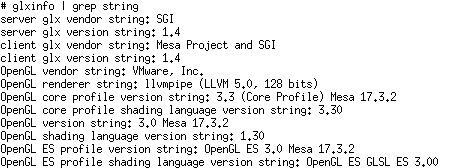
\includegraphics[scale=0.75]{img/llvmpipe-glspecs.png}
  \caption{OpenGL specs}
  \label{fig:llvmpipe-glspecs}
\end{figure}
Some benchmarks were run to compare llvmpipe against the classic softpipe software
rasterizer and the AMD Radeon HD6480. Table \ref{tab:glmark2_x86} shows how much
the LLVM code optimizer improves the performance for rendering:

\begin{table}[h!]
  \begin{center}
    \caption{Results of GLMark2 and GLMark2-es2 benchmarks on x86\_64}
    \label{tab:glmark2_x86}
    \begin{tabular}{ c |c c }
    & {GLMark2} & {GLMark2-es2} \\
    \hline
    Radeon HD6480 & 156 & 156 \\
    llvmpipe & 47 & 52 \\
    softpipe & 3 & 3 \\
    \end{tabular}
  \end{center}
\end{table}


\subsubsection*{ARM}
In order to test LLVM for ARM architecture, Raspberry Pi 2 and Raspberry Pi 3
development boards were used. For the case of the Raspberry Pi 3, the 32-bit
defconfig was selected.

\begin{table}[h!]
  \begin{center}
    \caption{Raspberry Pi 2 and 3 Hardware Specifications}
    \label{tab:rpi_specs}
    \begin{tabular}{c c c c c }
    Board & Family & SoC & CPU & GPU \\
    \hline
    RPi 2 & BCM2709 & BCM2836 @ 900 MHz & ARMv7 Cortex-A7 (Quad Core) & VC4 \\
    RPi 3 & BCM2710 & BCM2837 @ 1.2 GHz & ARMv8 Cortex-A53 (Quad Core) & VC4 \\
    \end{tabular}
  \end{center}
\end{table}
Raspberry Pi only supports OpenGL ES, so only GLMark2-es2 could be tested. When
trying to execute {\fontfamily{qcr}\selectfont glmark2} the following errors are
obtained:\\\\
{\fontfamily{qcr}\selectfont Error: GLX version >= 1.3 is required}\\\\
{\fontfamily{qcr}\selectfont Error: Error: Couldn't get GL visual config}\\\\
{\fontfamily{qcr}\selectfont Error: main: Could not initalize canvas}\\\\


\begin{table}[h!]
  \begin{center}
    \caption{Results of GLMark2-es2 for ARM}
    \label{tab:glmark2_ARM}
    \begin{tabular}{c|c}
    & {GLMark2-es2} \\
    \hline
    RPi2 softpipe & 0\\
    RPi2 llvmpipe & 0\\
    RPi3 (32-bit) softpipe & 0\\
    RPi3 (32-bit) llvmpipe & 11\\
    \end{tabular}
  \end{center}
\end{table}
Table \ref{tab:glmark2_ARM} shows an improvement in rendering when LLVM is used,
and also the higher computing power of the Cortex-A53 microprocessor.

\subsubsection*{AArch64}
Buildroot offers a defconfig to install a 64-bit system on the Raspberry Pi 3
(raspberrypi3\_64\_defconfig). There is a little improvement in rendering with
respect to the 32-bit version:
\begin{table}[h!]
  \begin{center}
    \caption{Results of GLMark2-es2 for AArch64}
    \label{tab:glmark2_AArch64}
    \begin{tabular}{c|c}
    & {GLMark2-es2} \\
    \hline
    RPi3 (64-bit) softpipe & 0\\
    RPi3 (64-bit) llvmpipe & 13\\
    \end{tabular}
  \end{center}
\end{table}
\subsection*{Considerations}
\begin{itemize}
    \item By default, the defconfigs for Raspberry Pi present in Buildroot have
    /dev management set to {\fontfamily{qcr}\selectfont Dynamic using devtmps only}.
    This must be changed to {\fontfamily{qcr}\selectfont Dynamic using devtmps +
    eudev} in order to allow Linux kernel to load modules dyamically, such as the
    VC4 device driver.

    \item To load VC4 device driver, assuming that the {\fontfamily{qcr}\selectfont
    /boot} partition has the {\fontfamily{qcr}\selectfont overlays/} directory with
    its dtbo files inside, the next options must be configured:
    \begin{itemize}
      \item Add cma=256M to cmdline.txt
      \item Set gpu\_mem/gpu\_mem\_1024 to 256 in config.txt
      \item Add dtoverlay=vc4-kms-v3d to config.txt
    \end{itemize}

    This steps allows to load the VC4 driver correctly, however it is not yet
    working well with X. When trying to execute any {\fontfamily{qcr}\selectfont
    glx} command, such as {\fontfamily{qcr}\selectfont glxinfo} or
    {\fontfamily{qcr}\selectfont glxgears}, it returns the following error:\\\\
    {\fontfamily{qcr}\selectfont Error: couldn't find RGB GLX visual or fbconfig}

    Possible causes:
    \begin{itemize}
      \item Mesa is not installing libglx.so in {\fontfamily{qcr}\selectfont
      /usr/lib/xorg/modules/extensions/}.
      \item Mesa 3D package in Buildroot states that a vanilla kernel 4.5+ must
      be used with Gallium VC4 (defconfig uses kernel from raspberrypi's Github).
      However, even in this case or using Eric Anholt's kernel\footnote{https://github.com/anholt/mesa/wiki/VC4-complete-Raspbian-upgrade}
      the error persists.
    \end{itemize}


\end {itemize}

\subsection*{Next steps}
\begin{itemize}
  \item Enable dynamic linking for Mesa 3D. This is important because when building
        packages that link against LLVM libraries the same problem may arise.
  \item For Raspberry Pi:
    \begin{itemize}
      \item Activate glx.
      \item Activate OpenGL for VC4.
    \end{itemize}
  \item Prepare next patch series:
  \begin{itemize}
    \item Provide an option to install full host-llvm.
    \item Activate OpenCL.
    \item Activate Clang (needs full host-llvm installed).
    \item Add support for more targets.
  \end{itemize}
\end{itemize}

\newpage
\section*{Update - 9 March 2018}

\subsection*{Full host-llvm}
After having investigated why Mesa 3D was not able to link dynamically against
libLLVM.so, it was found that the bug in llvm-config presented in section \textbf{Mesa 3D}
occurs when the option LLVM\_LINK\_LLVM\_DYLIB is not enabled. The purpose of this
option is to generate a single shared library (libLLVM.so) and link LLVM tools
dynamically with it.\\\\
A priori, as llvm-tblgen and llvm-config are the only necessary tools for the host
(llvm-tblgen to cross-compile LLVM for the target and llvm-config to provide linking
options to packages that link against LLVM libraries), it was decided to do a
minimal host-llvm installation. However, to get the correct output from llvm-config
it must be linked with libLLVM.so (host-variant), so this library must also be built.
Because of this, the first approach changed and the first patch of the series
(package/llvm: new host package) will provide a full installation of LLVM (tools
and libraries). This approach will avoid conflicts for packages linking with
LLVM libraries and will also facilitate the integration of Clang front-end, which
will be provided in a future patch series.

\subsection*{PATCH v3}
The PATCH v3 series\footnote{http://lists.busybox.net/pipermail/buildroot/2018-March/215490.html}
sent to the Buildroot mailing list on the $9^{th}$ March contains the following
6 commits:
\begin{itemize}
  \item {[PATCH v3 1/6]} package/llvm: new host package
  \item {[PATCH v3 2/6]} package/llvm: enable target variant
  \item {[PATCH v3 3/6]} package/llvm: enable AMDGPU
  \item {[PATCH v3 4/6]} package/mesa3d: enable llvm support
  \item {[PATCH v3 5/6]} package/llvm: enable ARM
  \item {[PATCH v3 6/6]} package/llvm: enable AArch64
\end{itemize}

\newpage
\section*{Update - 29 March 2018}

\subsection*{New series to enable OpenCL}
Once LLVM was tested working on the three more common architectures (x86, ARM and
Aarch64), the next goal was activating OpenCL support. This task involved
multiple steps, as there are many dependencies that need to be satisfied.\\\\
OpenCL is an API enabling general purpose computing on GPUs (GPGPU) and other
devices (CPUs, DSPs, FPGAs, ASICs, etc.), being well suited for certain kinds of
parallel computations, such as hash cracking (SHA, MD5, etc.), image processing and
simulations.\\\\
OpenCL presents itself as a library with a simple interface:
\begin{itemize}
  \item Standarized API headers for C and C++
  \item The OpenCL library (libOpenCL.so), which is a collection of types and
  functions which all conforming implementations must provide.
\end{itemize}
The standard is made to provide many OpenCL platforms on one system, and each
platform can see various devices. Each device has certain compute characteristics
(number of compute units, optimal vector size, memory limits, etc). The OpenCL
standard allows to load OpenCL kernels which are pieces of C99-like code that is
JIT-compiled by the OpenCL implementations (most of them rely on LLVM to work),
and execute these kernels on the target hardware. Functions are provided to
compile the kernels, load them, transfer data back and forth from the target
devices, etc.\\\\
There are multiple open source OpenCL implementations for Linux:
\begin{itemize}
  \item \textbf{Clover (Computing Language over Gallium)}\\\\
  It is a hardware independent OpenCL API implementation that works with Gallium
  Drivers (hardware dependent userspace GPU drivers) which was merged into Mesa 3D
  in 2012. It currently supports OpenCL 1.1 and it is close to 1.2 It has the
  following dependencies:
    \begin{itemize}
      \item \textbf{libclang}: provides an OpenCL C compiler frontend and generates LLVM IR.
      \item \textbf{libLLVM}: LLVM IR optimization passes and hardware dependent code
      generation.
      \item \textbf{libclc}: implementation of the OpenCL C standard library in LLVM IR
      bitcode providing device builtin functions. It is linked at runtime.
    \end{itemize}
  \item \textbf{Pocl}\\\\
  This implementation is OpenCL 1.2 standard compliant and supports some 2.0
  features. The major goal of this project is to improve performance portability
  of OpenCL programs, reducing the need for target-dependent manual optimizations.
  Pocl currently supports many CPUs (x86, ARM, MIPS, PowerPC), ASPIs(TCE/TTA),
  NVIDIA GPUs via CUDA (experimental), HSA-supported GPUs and multiple private
  off-tree targets. It also works with libclang and libLLVM but it has its own
  Pocl Builtin Lib (instead of using libclc).
  \item \textbf{Beignet}\\\\
  It targets Intel GPUs (HD and Iris) starting with Ivy Bridge, and offering
  OpenCL 2.0 support for Skylake, Kaby Lake and Apollo Lake.
  \item \textbf{ROCm}\\\\
  This implementation by AMD targets ROCm (Radeon Open Compute) compatible
  hardware\footnote{https://github.com/RadeonOpenCompute/ROCm} (HPC/Hyperscale),
  providing OpenCL 1.2 API with OpenCL C 2.0. It has become open source in May
  2017.
\end{itemize}

\begin{table}[h!]
  \begin{center}
    \caption{Open source OpenCL implementations}
    \label{tab:opencl_implementations}
    \begin{tabular}{c|c|c}
    Project & Version & Hardware \\
    \hline
    Clover & 1.1 & AMD\\
    Pocl & 1.2 & CPU, NVIDIA\footnote{Needs propietary drivers}, AMD\footnote{HSA
    compatible hardware}, TCE/TTA\\
    Beignet & 2.0 & Intel\\
    ROCm OpenCL & 1.2 & AMD\footnote{ROCm compatible hardware}\\
    \end{tabular}
  \end{center}
\end{table}
Because of this fragmentation concerning OpenCL implementations (without taking
into account the propietary ones) there exists a program that allows multiple
implementations to co-exist on the same sytem: OpenCL ICD (Installable Client
Driver). It needs the following components to work:
\begin{itemize}
  \item \textbf{libOpenCL.so (ICD loader)}: this library dispatches the OpenCL
  calls to OpenCL implementations.
  \item \textbf{/etc/OpenCL/vendors/*.icd}: these files tell the ICD loader which
  OpenCL implementations (ICDs) are installed on the sytem. Each file has a single
  line containing the name of the shared library with the implementation.
  \item \textbf{One or more OpenCL implementations (the ICDs)}: the shared libraries
  pointed by the .icd files.
\end{itemize}

\newpage
\subsection*{Preparation of the new series}
Considering that the available system for tests has an AMD Radeon Dual Graphics
GPU (integrated HD6480G + dedicated HD7450M) and that Mesa 3D is already present
in Buildroot, it was decided to work with the OpenCL implementation provided by
Clover. The diagram in Fig.\ref{fig:clover} shows which are the necessary
components to set up the desired OpenCL environment and how they interact with
each other.

\begin{figure}[H]
\centering
  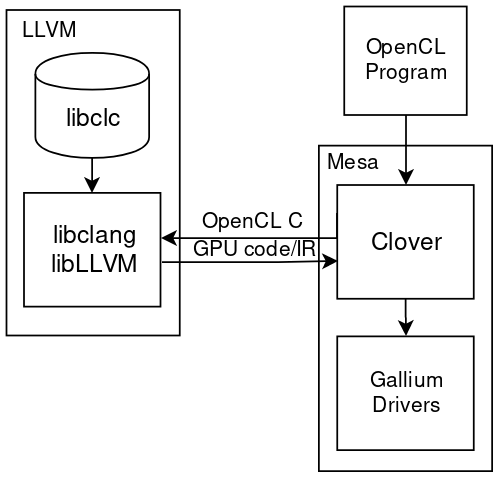
\includegraphics[scale=0.65]{img/clover.png}
  \caption{Clover OpenCL implementation}
  \label{fig:clover}
\end{figure}

\subsubsection*{Clang for host}
The first step was providing Clang frontend for the host, as it is necessary for
building libclc because this library is written in OpenCL C and some functions
are implemented directly in LLVM IR. Clang will transform .cl and .ll source
files into LLVM IR bitcode (.bc) by calling llvm-as (the LLVM assembler).\\\\
Regarding the Makefile for building host-clang, the path to host's llvm-config
must be specified. This is necessary because Clang is thought to be built as a
tool inside LLVM's tree (LLVM\_SOURCE\_TREE/tools/clang) but Buildroot manages
packages individually, so Clang's code source cannot be downloaded inside LLVM's
tree.\\\\
Having Clang installed on the host is not only useful for building libclc, it
provides an alternative to GCC, what enables the possibility of creating a new
toolchain based on it.

\newpage
\subsubsection*{Clang for target}
When trying to cross-compile Clang some problems were encountered, so it was
decided to work with ARM architecture in order to make sure that a build on x86
was successful not just because of binary compatibility. The main issues were the
following ones:
\begin{itemize}
  \item \textbf{llvm-tblgen}\\\\
  When trying to cross-compile Clang, the build broke with the following error:\\\\
  {\fontfamily{qcr}\selectfont llvm-tblgen: cannot execute binary file: Exec
  format error}\\\\
  This means that llvm-tblgen from STAGING\_DIR (cross-compiled) was trying to be
  executed on the host machine. Because of this, it was necessary to copy
  llvm-tblgen from host to STAGING\_DIR/usr/bin. This is the same kind of problem
  that arised with llvm-config, which was explained before.

  \item \textbf{llvm-config}\\\\
  It is necessary to specify the path to llvm-config installed in STAGING\_DIR:\\\\
  {\fontfamily{qcr}\selectfont -DLLVM\_CONFIG:FILEPATH=\$(STAGING\_DIR)/usr/bin/llvm-config}

  \item \textbf{Shared libs}\\\\
  When Clang was built for the host, it generated multiple static libraries
  (libclangAST.a, libclangFrontend.a, libclangLex.a, etc.) and finally a shared
  object (libclang.so) containing all of them. However, when building for the
  target, it generated multiple shared libraries and finally libclang.so. This
  resulted in the following error when trying to use tools that link with
  libOpenCL, which statically links with libclang (e.g, clinfo):\\\\
  {\fontfamily{qcr}\selectfont
  \$ CommandLine Error: Option 'track-memory' registered more than once!\\
  \$ LLVM ERROR: inconsistency in registered CommandLine options
  }\\\\
  The solution to this was specifying explicitely to the CMake infrastructure that
  shared libraries should not be built:\\\\
  {\fontfamily{qcr}\selectfont CLANG\_CONF\_OPTS += -DBUILD\_SHARED\_LIBS=OFF}
\end{itemize}

\subsubsection*{libclc}
This library provides an implementation of the library requirements of the
OpenCL C programming language, as specified by the OpenCL 1.1 specification.
It is designed to be portable and extensible, as it provides generic
implementations of most library requirements, allowing targets to override them
at the granularity of individual functions, using LLVM intrinsics for example.
It currently supports AMDGCN, R600 and NVPTX targets.\\\\
There is a particular problem with libclc: when OpenCL programs call clBuildProgram
function\footnote{https://www.khronos.org/registry/OpenCL/sdk/2.0/docs/man/xhtml/clBuildProgram.html}
in order to compile and link a program (generally an OpenCL kernel) from source
during execution, they require clc headers to be located in /usr/include/clc.
This is not possible because Buildroot does not copy /usr/include from STAGING\_DIR
to the target as the embedded platform is not intended to store development files,
mainly because there is no compiler installed on it. But since OpenCL works with
libLLVM to do code generation, a place to store clc headers must be found.\\\\
The file that adds the path to libclc headers is invocation.cpp, located at
src/gallium/state\_trackers/clover/llvm, inside Mesa's source tree:\\

\begin{lstlisting}[language=C++,caption={Extract from invocation.cpp},captionpos=b]
// Add libclc generic search path
c.getHeaderSearchOpts().AddPath(LIBCLC_INCLUDEDIR,
                                clang::frontend::Angled,
                                false, false);
// Add libclc include
c.getPreprocessorOpts().Includes.push_back("clc/clc.h");
\end{lstlisting}

Variable LIBCLC\_INCLUDEDIR is defined in Mesa's configure.ac:\\

\begin{lstlisting}[language=sh,caption={Extract from configure.ac},captionpos=b]
LIBCLC_INCLUDEDIR=`$PKG_CONFIG --variable=includedir libclc`
LIBCLC_LIBEXECDIR=`$PKG_CONFIG --variable=libexecdir libclc`
\end{lstlisting}

Currently, header files are being copied to /usr/include/clc once the root
filesystem is generated, but this solution only works for testing because systems
generated with Buildroot must work directly after being built. The next step
is to test if LIBCLC\_INCLUDEDIR can be overwritten by specifying another path
instead of using pkg-config.

\subsubsection*{clinfo}
Clinfo is a simple command-line application that enumerates all possible (known)
properties of the OpenCL platform and devices available on the system. It tries
to output all possible information, including those provided by platform-specific
extensions.\\\\
This application is built with a simple Makefile, so when creating the package
for Buildroot it was sufficient to call the generic-package infrastructure. The
main purposes of it are:
\begin{itemize}
  \item Verifying that the OpenCL environment is set up correctly. If clinfo
  cannot find any platform or devices (or fails to load the OpenCL dispatcher
  library), chances are high no other OpenCL application will run.
  \item Verifying that the OpenCL development environment is set up correctly:
  if clinfo fails to build, chances are high no other OpenCL application will
  build.
  \item Reporting the actual properties of the available device(s).
\end{itemize}
Once installed on the target, clinfo successfully found Clover and the devices
available to work with it, providing the following output:\\
\begin{lstlisting}[language=sh,caption={Output of clinfo},captionpos=b,keywords={}]
Number of platforms                   1
Platform Name                         Clover
Platform Vendor                       Mesa
Platform Version                      OpenCL 1.1 Mesa 17.3.7
Platform Profile                      FULL_PROFILE
Platform Extensions                   cl_khr_icd
Platform Extensions function suffix   MESA

Platform Name                         Clover
Number of devices                     2
Device Name                           AMD SUMO (DRM 2.50.0 / 4.14.0, LLVM 5.0.1)
Device Vendor                         AMD
Device Vend                           0x1002
Device Version                        OpenCL 1.1 Mesa 17.3.7
Driver Version                        17.3.7
Device OpenCL C Version               OpenCL C 1.1
Device Type                           GPU
Device Profile                        FULL_PROFILE
Device Available                      Yes
Compiler Available                    Yes
Max compute units                     1
Max clock frequency                   0MHz
Max work item dimensions              3
Max work item sizes                   256x256x256
Max work group size                   256
Preferred work group size multiple    64
\end{lstlisting}
\subsubsection*{Piglit}
Piglit is a collection of automated tests for OpenGL and OpenCL implementations.
The goal of this project is to help improving the quality of open source OpenGL and
OpenCL drivers by providing developers with a simple means to perform regression
tests.\\\\
Once Clover was installed on the target system, it was decided to run Piglit in
order to verify Mesa's OpenCL implementation conformance, taking the Buildroot
packaging from Romain Naour's series
\footnote{http://lists.busybox.net/pipermail/buildroot/2018-February/213601.html}:
\begin{itemize}
  \item {[PATCH v2 1/3]} package/python-numpy: add host variant for piglit
  \item {[PATCH v2 2/3]} package/waffle: new package
  \item {[PATCH v2 3/3]} package/piglit: new package
\end{itemize}
To run the OpenCL test suite, the following command must be executed:
\begin{lstlisting}[language=sh]
  piglit run tests/cl results/cl
\end{lstlisting}
The results are written in JSON format, and can be converted to HTML by running:
\begin{lstlisting}[language=sh]
  piglit summary html --overwrite summary/cl results/cl
\end{lstlisting}
\begin{figure}[H]
\centering
  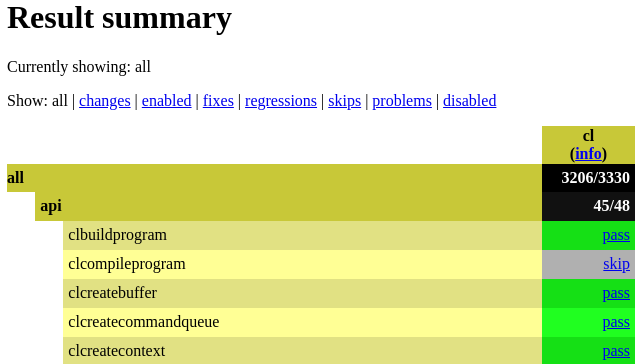
\includegraphics[scale=0.65]{img/html_output.png}
  \caption{OpenCL Test Suite results in HTML}
  \label{fig:html_output}
\end{figure}
The results of the OpenCL test suite were the following ones:
\begin{table}[h!]
  \begin{center}
    \caption{Piglit OpenCL Test Suite on AMD SUMO + AMD CAICOS}
    \label{tab:piglit_opencl}
    \begin{tabular}{c|c|c|c|c}
    Total & Skip & Pass & Fail & Crash \\
    \hline
    704 & \color{blue}{94} & \color{green}{541} & \color{red}{60} & 9
    \end{tabular}
  \end{center}
\end{table}\\
Most of the tests that failed can be classified in the following categories:
\begin{itemize}
  \item Program build with optimization options for OpenCL C 1.0/1.1+
  \item Global atomic operations (add, and, or, max, etc.) using a return variable
  \item Floating point multiply-accumulate operations
  \item Some builtin shuffle operations
  \item Global memory
  \item Image read/write 2D
  \item Tail calls
  \item Vector load
\end{itemize}
Some failures are due to missing hardware support for particular operations, so
it would be useful to run Piglit with a more recent GPU using radeonsi Gallium
driver in order to compare the results. It would also be interesting to test
with both GPUs which packages can benefit from OpenCL support using Clover.
\subsection*{PATCH v4}
The PATCH v4 series\footnote{http://lists.busybox.net/pipermail/buildroot/2018-March/216772.html}
sent to the Buildroot mailing list on the $29^{th}$ March contains the following
11 commits:
\begin{itemize}
  \item {[PATCH v4 1/11]} package/llvm: new host package
  \item {[PATCH v4 2/11]} package/llvm: enable target variant
  \item {[PATCH v4 3/11]} package/llvm: enable AMDGPU
  \item {[PATCH v4 4/11]} package/mesa3d: enable llvm support
  \item {[PATCH v4 5/11]} package/llvm: enable ARM
  \item {[PATCH v4 6/11]} package/llvm: enable AArch64
  \item {[PATCH v4 7/11]} package/clang: new host package
  \item {[PATCH v4 8/11]} package/clang: enable target variant
  \item {[PATCH v4 9/11]} package/libclc: new package
  \item {[PATCH v4 10/11]} package/mesa3d: enable OpenCL support
  \item {[PATCH v4 11/11]} package/clinfo: new package
\end{itemize}

\newpage
\section*{Update - 13 April 2018}
A Buildroot hackathon gathering the core developers of the project took place
during the March 31-April 2 weekend in Paris. After an extensive review of the
v4 series by Romain Naour and Thomas Petazzoni, the following feedback was
received:
\begin{itemize}
  \item There is no need to have a visible Config.in.host option for host-llvm,
  as it is merely needed as a build dependency of the target llvm.
  \item Activate CCACHE, considering that Buildroot has CCACHE support and it
  is useful considering the size of LLVM.
  \item LLVM needs a toolchain with thread and C++ support.
  \item Some options are already passed by the CMake package infrastructure of
  Buildroot, so they are not necessary in llvm.mk, such as CMAKE\_INSTALL\_PREFIX
  and -G "Unix Makefiles".
  \item Manage LLVM\_TARGETS\_TO\_BUILD in a more extensible way to add more backends.
  \item Support for ARM and Aarch64 architectures should go directly in the
  first patch of the series.
  \item Clang binaries must be removed from the target, as there are no development
  files (headers) and other build tools.
\end{itemize}
Taking into account all these considerations, the next version of the series
was prepared.

\subsection*{PATCH v5}
The PATCH v5 series\footnote{http://lists.busybox.net/pipermail/buildroot/2018-April/218023.html}
sent to the Buildroot mailing list on the $4^{th}$ April contains the  following
7 commits:
\begin{itemize}
  \item {[PATCH v5 1/7]} package/llvm: new package
  \item {[PATCH v5 2/7]} package/llvm: enable AMDGPU
  \item {[PATCH v5 3/7]} package/mesa3d: enable llvm support
  \item {[PATCH v5 4/7]} package/clang: new package
  \item {[PATCH v5 5/7]} package/libclc: new package
  \item {[PATCH v5 6/7]} package/mesa3d: enable OpenCL support
  \item {[PATCH v5 7/7]} package/clinfo: new package
\end{itemize}
\newpage
\subsection*{Achievements}
LLVM package\footnote{http://lists.busybox.net/pipermail/buildroot/2018-April/218058.html}
and LLVM support for Mesa 3D\footnote{http://lists.busybox.net/pipermail/buildroot/2018-April/218060.html}
were commited to Buildroot's master branch on the $4^{th}$ April.
\subsection*{Bug fixing}
Thanks to Buildroot autobuilders\footnote{http://autobuild.buildroot.org/} it was
possible to detect some bugs that were not found during development. These
autobuilders are machines that select a target architecture, a toolchain, some
packages randomly and try to build that configuration. There is a daily report
containing the results of the autobuilders that shows which packages failed to
build for a particular configuration. It is also possible to analyze the build
log and the .config so that bugs can be corrected quickly.

\subsubsection*{GCC Bug 64735}
Autobuild:\\\\
http://autobuild.buildroot.net/results/ada497f6a8d20fa1a9adb2b17a138d7b726a6cdc/\\\\
Extract from build-end.log:
\begin{lstlisting}[language=sh,keywords={}]
output/build/llvm-5.0.1/lib/Support/ThreadPool.cpp:14:0:
output/build/llvm-5.0.1/include/llvm/Support/ThreadPool.h: In member function
'std::shared_future<void> llvm::ThreadPool::async(Function&&, Args&& ...)':
output/build/llvm-5.0.1/include/llvm/Support/ThreadPool.h:54:75: error:
return type 'class std::shared_future<void>' is incomplete inline
std::shared_future<void> async(Function &&F, Args &&... ArgList)
\end{lstlisting}
Fix (Thomas Petazzoni):\\\\
This autotest was targeting an ARM926EJ-S processor (ARMv5 architecture). LLVM
uses std::shared\_future, which until gcc 7.x is not available on architectures
that do not provide lock-free atomics: https://gcc.gnu.org/bugzilla/show\_bug.cgi?id=64735.
Buildroot already has a BR2\_TOOLCHAIN\_HAS\_GCC\_BUG\_64735 option to handle such a
case, so this new dependency must be added to LLVM. It will make sure LLVM does
not get built on ARMv5 platforms using a GCC older than 7.x.\\\\
Commit: http://lists.busybox.net/pipermail/buildroot/2018-April/218267.html

\subsubsection*{Shared libraries}
Autobuild:\\\\
http://autobuild.buildroot.net/results/301c454c6eab802405a268f4713a574d1c366892/\\\\
Extract from build-end.log:
\begin{lstlisting}[language=sh,keywords={}]
Linking CXX shared library ../../lib/libLTO.so
arm-buildroot-linux-musleabihf/bin/ld: attempted static link of dynamic object
`../../lib/libLLVM-5.0.so' collect2: error: ld returned 1 exit status
\end{lstlisting}
Fix:\\\\
Buildroot provides an option to build and use only static libraries on the target
system. LLVM will not work in this case as it generates shared libraries. Because
of this, the package should not be available if BR2\_STATIC\_LIBS is set.\\\\
Commit: http://lists.busybox.net/pipermail/buildroot/2018-April/218550.html

\subsubsection*{BR2\_USE\_WCHAR}
Autobuild:\\\\
This error was detected locally.\\\\
Extract from log:
\begin{lstlisting}[language=sh]
output/build/llvm-5.0.1/include/llvm/Support/ConvertUTF.h:203:53:
error: ‘std::wstring’ has not been declared
bool ConvertUTF8toWide(llvm::StringRef Source, std::wstring &Result);
\end{lstlisting}
Fix:\\\\
LLVM uses std::wstring, so a toolchain with wchar support is necessary.\\\\
Commit: http://lists.busybox.net/pipermail/buildroot/2018-April/218549.html

\subsubsection*{Gallium R600 with LLVM needs libelf}
Autobuild:\\\\
http://autobuild.buildroot.org/results/8845ff0f28d3273ebe884126b85cd7c4a905d81b/\\\\
Extract from log:
\begin{lstlisting}[language=sh,keywords={}]
checking for EXPAT... yes
checking for RADEON... yes
configure: error: r600 requires libelf when using llvm
\end{lstlisting}
Fix:\\\\
Gallium R600 driver needs libelf when Mesa 3D is built with LLVM support. Because
of this, the toolchain must use either uClibc or glibc, as musl is not currently
compatible with elfutils.\\\\
Commit: http://lists.busybox.net/pipermail/buildroot/2018-April/218985.html
\newpage
\subsubsection*{llvm-config's RPATH}
Autobuild:\\\\
http://autobuild.buildroot.net/results/b81c12d529c66a028e2297ea5ce1d6930324fa69/\\\\
Extract from log:
\begin{lstlisting}[language=sh,keywords={}]
checking for llvm-config...
output/host/x86_64-buildroot-linux-uclibc/sysroot/usr/bin/llvm-config
/output/host/x86_64-buildroot-linux-uclibc/sysroot/usr/bin/llvm-config:
error while loading shared libraries: libc.so.0: cannot open shared object
file: No such file or directory
\end{lstlisting}
Fix:\\\\
In this case, Mesa 3D failed to build because it could not execute correctly
llvm-config. The problem is the following: llvm-config (host version installed in
STAGING\_DIR) is not being able to link correctly with the libc of the host system.
This happens in the following scenario: target architecture = host architecture
(normally x86\_64) and target's libc different from host's libc (normally glibc).\\\\
As the RPATH of llvm-config specifies \$ORIGIN/../lib (seen using readelf -d
llvm-config) and the binary is located in STAGING\_DIR/usr/bin, it tries to link
with the libc of the target, resuting in the error displayed above.\\\\
It was found that function {\fontfamily{qcr}\selectfont llvm\_setup\_rpath} in
AddLLVM.cmake sets this RPATH, but it just returns in case CMAKE\_INSTALL\_RPATH
is defined. So the final solution was passing HOST\_LLVM\_CONF\_OPTS += -DCMAKE\_INSTALL\_RPATH="\$(HOST\_DIR)/lib"
in llvm.mk, so that LLVM binaries compiled for the host always link with host's
libraries.\\\\
Commit: http://lists.busybox.net/pipermail/buildroot/2018-April/218938.html

\subsection*{Preparation of the new series}
After having fixed the bugs found by the autobuilders, the OpenCL series was
retaken, adding the following improvements:
\begin{itemize}
  \item In order to cross-compile Clang, now llvm-tblgen from the host is used.
  llvm-tblgen is no longer copied to STAGING\_DIR/usr/bin.
  \item libclc headers are now installed to /usr/local/include by using the
  --includedir option in libclc.mk. This directory is not removed by Buildroot
  when generating the target root filesystem.
  \item Some missing dependencies were propagated.
\end{itemize}
\newpage
\subsection*{PATCH v6}
The PATCH v6 series\footnote{http://lists.busybox.net/pipermail/buildroot/2018-April/218849.html}
sent to the Buildroot mailing list on the $11^{th}$ April contains the following
4 commits:
\begin{itemize}
  \item {[PATCH v6 1/4]} package/clang: new package
  \item {[PATCH v6 2/4]} package/libclc: new package
  \item {[PATCH v6 3/4]} package/mesa3d: enable OpenCL support
  \item {[PATCH v6 4/4]} package/clinfo: new package
\end{itemize}

\newpage
\section*{Update - 23 April 2018}
\subsection*{OpenCL for Broadcom Videocore IV}
The next goal was adding OpenCL support for the Broadcom Videocore IV GPU in
Buildroot. This is an interesting feature considering that this GPU is embedded
in all Raspberry Pi models.
\subsubsection*{Videocore IV architecture}
The VC4 has multiple instances of a special purpose floating-point shader processor,
called a Quad Processor (QPU). The QPU is a 16-way SIMD processor, where each
processor has two vector floating point ALUs which carry out multiply and
non-multiply operations in parallel with single instruction cycle latency.
Internally the QPU is a 4-way SIMD processor multiplexed 4x over four cycles
\begin{figure}[H]
\centering
  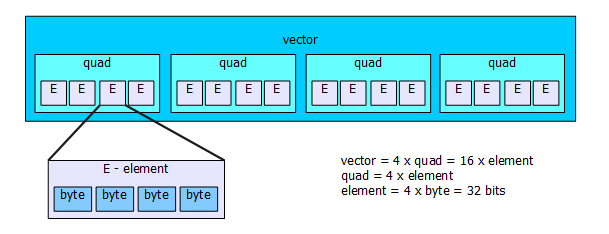
\includegraphics[scale=0.85]{img/vc4_qpu_vector.png}
  \caption{QPU data model}
  \label{fig:html_output}
\end{figure}
QPU is SIMD architecture (Single Instruction, Multiple Data), this means that one
instruction operates on a vector of elements. When looking from the programmer's
point of view, it processes a vector of 16 elements each 32-bits long. If physical
structure is taken into account, a QPU processes only a 4-element vector (quad).
By repeating the instruction 4 times for consecutive quads in a 16-element vector,
it provides a virtual SIMD-16.\\\\
QPUs are organized into groups of up to four, termed slices, which share certain
common resources: each slice shares an instruction cache, a Special Function Unit
(for recip/recipsqrt/log/exp functions), one or two Texture and Memory lookup units
and Interpolation units. As the Videocore IV has 3 slices of 4 QPUs each one,
it provides 12 QPUs and 3 SFUs, which makes this GPU an interesting option for
solving problems that present data level parallelism. Broadcom claims a computational
power of 24 GFLOPs, which comes out from the following equation:\\\\
250 MHz (Clock Rate) * 4-Way SIMD * 2 Asymmetric ALUs * 12 QPUs = 24 GFLOPs
\begin{figure}[H]
\centering
  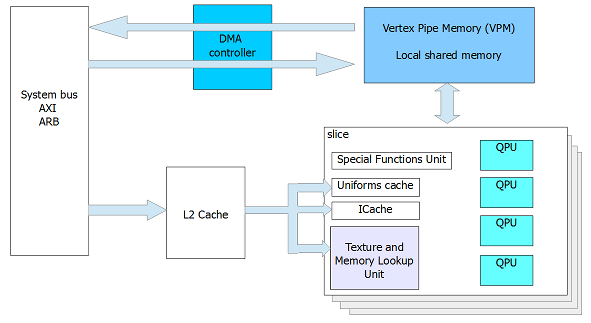
\includegraphics[scale=1]{img/vc4_qpu.png}
  \caption{Simplified architecture of the Videocore IV}
  \label{fig:html_output}
\end{figure}

\subsubsection*{VC4CL}
There is an open source project called VC4CL\footnote{https://github.com/doe300/VC4CL/wiki}
that provides an implementation that supports the EMBEDDED PROFILE (trimmed
version of the default FULL PROFILE) of the OpenCL 1.2 standard for the VideoCore
IV GPU. This implementation consists of:
\begin{itemize}
    \item The VC4CL OpenCL runtime library, running on the CPU to compile,
    run and interact with OpenCL kernels.
    \item The VC4C compiler, converting OpenCL kernels into machine code. This
    compiler also provides an implementation of the OpenCL built-in functions.
    \item The VC4CLStdLib, the platform-specific implementation of the OpenCL C
    standard library, it is linked with the kernel via VC4C.
\end{itemize}
The {\fontfamily{qcr}\selectfont cl\_khr\_icd} extension is supported to allow
VC4CL to be found by an installable client driver loader (ICD). As explained
before, it allows VC4CL to be used in parallel with other OpenCL implementations.
\\\\
Not supported features:
\begin{itemize}
  \item 64-bit data-types (long and double via {\fontfamily{qcr}\selectfont cl\_khr\_fp64})
  are unsupported, since the Videocore IV GPU only provides 32-bit instructions.
  \item The {\fontfamily{qcr}\selectfont cl\_khr\_fp16} half floating-point type is
  also not supported.
  \item Images (WIP).
  \item Any application which requires a work-group with more than 12 work-items.
  \item Using VC4CL in combination with other applications using the VideoCore IV
  GPU (e.g. the VC4 Mesa driver) is untested and can cause issues on both sides.
\end{itemize}

\subsubsection*{VC4CL package for Buildroot}
In order to install VC4CL, VC4CLStdLib and VC4C are needed. As these projects
are thought to be installed natively on top of a Raspbian distribution, some changes
were made to cross-compile them under the Buildroot environment.\\\\
When instaling VC4CLStdLib, it was necessary to change the location
of its header files to /usr/local/include, as they are required on runtime by the
VC4C compiler and, as explained before, Buildroot removes the /usr/include
directory from the target filesystem.\\\\
One particularity of this implementation is that it calls Clang binaries in order
to compile OpenCL kernels on the target instead of linking with libclang, as most
OpenCL implementations do. Even if the package was tested and working, this fact
prevents this patch series from being sent to the Buildroot mailing list, as the
mantainers do not allow a compiler to be installed on the target.\\\\
The VC4C package has the same dependencies as Clang, but also needs VC4CLStdLib
and Raspberry Pi Userland, the latter providing EGL and KHR headers. Regarding
VC4C's Makefile, two hooks were added: one to copy Clang binaries to /usr/bin
(Clang's Makefile removes them from the target) and another one to install a
precompiled header (VC4CLStdLib.h.pch) that is built during VC4C's compilation
to /usr/local/include/vc4cl-stdlib, as it is a runtime dependency of VC4CL.\\\\
VC4C gives the user the possibility of choosing among three different frontends:
LLVM IR Parser, SPIR-V Reader or LLVM Library:
\begin{table}[h!]
  \begin{center}
    \caption{Frontends}
    \label{tab:piglit_opencl}
    \begin{tabular}{c|c|c|c}
    \textbf{Frontend}  & \textbf{LLVM IR Parser} & \textbf{SPIR-V Reader} & \textbf{LLVM Library} \\
    \hline
    Input formats & LLVM IR text & SPIR-V text/bin & LLVM IR text/bin \\
    Speed &	Slow &	Fast &	Faster \\
    Supported LLVMs &	Standard/SPIRV &	SPIRV &	Standard/SPIRV \\
    Runtime Deps &	Clang &	SPIRV-LLVM Clang  &	Clang, libLLVM \\
    Development Deps &	- & SPIRV-Tools	& LLVM headers \\
    Configuration &	LLVMIR\_FRONTEND &	SPIRV\_FRONTEND &	LLVMLIB\_FRONTEND\\
    Supports linking & No & Yes & No
    \end{tabular}
  \end{center}
\end{table}\\
The LLVM Library frontend was selected, as its dependencies are already packaged
in Buildroot and this is also the suggested option by the creator of the project.
It suffices to give the path to llvm-config installed in STAGING\_DIR in vc4c.mk
so that libLLVM.so can be found.\\\\
It is important to remark that CMakeLists.txt of VC4C was patched because it
needs to find and execute Clang during configuration (which can only be achieved
by passing the path to host's Clang) but needs the path to target's Clang for
runtime kernel compilation.\\\\
The last step was packaging VC4CL. This package needs ocl-icd as a dependency, so
this package was also created and VC4CL was built with ICD support, so that VC4CL.icd
containing the path to libVC4CL.so was installed to /etc/OpenCL/vendors.

\subsubsection*{Testing VC4CL}
To verify that the OpenCL environment was correctly set up, clinfo was installed
and executed, obtaining the following output:
\begin{lstlisting}[language=sh,caption={Output of clinfo},captionpos=b,keywords={}]
Number of platforms                    1
Platform Name                         OpenCL for the Raspberry Pi VideoCore
                                      IV GPU
Platform Vendor                       doe300
Platform Version                      OpenCL 1.2 VC4CL 0.4
Platform Profile                      EMBEDDED_PROFILE
Platform Extensions                   cl_khr_il_program cl_khr_spir
                                      cl_altera_device_temperature
                                      cl_altera_live_object_tracking
                                      cl_khr_icd
                                      cl_vc4cl_performance_counters
Platform Extensions function suffix   VC4CL
Platform Name                         OpenCL for the Raspberry Pi VideoCore
                                      IV GPU
Number of devices                     1
Device Name                           VideoCore IV GPU
Device Vendor                         Broadcom
Device Vendor ID                      0xa5c
Device Version                        OpenCL 1.2 VC4CL 0.4
Driver Version                        0.4
Device OpenCL C Version               OpenCL C 1.2
Device Type                           GPU
Device Profile                        EMBEDDED_PROFILE
Device Available                      Yes
Compiler Available                    Yes
Linker Available                      No
Max compute units                     1
Max clock frequency                   250MHz
Device Partition                      (core)
Max number of sub-devices             0
Supported partition types             None
Max work item dimensions              3
Max work item sizes                   12x12x12
Max work group size                   12
Preferred work group size multiple    1
\end{lstlisting}
Something that called the attention during the execution of clinfo was the fact
that it took much more time than expected. This application calls
clCreateProgramWithSource() in order to create a program object receiving the
source code of an OpenCL kernel as input. This step involves calling Clang, which
results in a bottleneck when using a Cortex-A7 processor running at 900Mhz
(Raspberry Pi 2), considering that OpenCL programs are made to improve execution time.
\begin{lstlisting}[language=sh,caption={Clang invocation by clCreateProgramWithSource() },captionpos=b,keywords={}]
/usr/bin/clang -cc1 -triple spir-unknown-unknown  -O3 -ffp-contract=off
-cl-std=CL1.2 -cl-kernel-arg-info -cl-single-precision-constant
-Wno-undefined-inline -Wno-unused-parameter -Wno-unused-local-typedef
-Wno-gcc-compat -x cl -S -emit-llvm-bc -o /tmp/vc4c-DRbyiL
-include-pch /usr/local/include/vc4cl-stdlib/VC4CLStdLib.h.pch
\end{lstlisting}
Most OpenCL programs make use of this function, but compiling kernels on the
target is definitely not a viable solution. A better alternative is to compile
kernels on the host and use clCreateProgramWithBinary(). This function creates a
program object for a context, and loads specified binary data into the program
object. For this, OpenCL kernels must be compiled to LLVM bitcode by using host-clang:
\begin{lstlisting}[language=sh,caption={Compiling OpenCL C to LLVM bitcode},captionpos=b,keywords={}]
clang -cc1 -emit-llvm-bc -o kernel_pi.bc kernel_pi.cl
\end{lstlisting}
On the other side, the program must read the corresponding bitcode file and then
create the program by calling clCreateProgramWithBinary:
\begin{lstlisting}[language=C,caption={Example using clCreateProgramWithBinary},captionpos=b,showstringspaces=false]
FILE *fp;
char fileName[] = "./kernel_pi.bc";
size_t binary_size;
char *binary_buf;

/* Load kernel binary */
fp = fopen(fileName, "r");
if (!fp) {
        fprintf(stderr, "Could not read the kernel file: %s\n", fileName);
        exit(1);
}
binary_buf = (char *)malloc(MAX_BINARY_SIZE);
binary_size = fread(binary_buf, 1, MAX_BINARY_SIZE, fp);
fclose(fp);
...
...
clGetPlatformIDs(..
clGetDeviceIDs(...
clCreateContext(...
clCreateCommandQueue(...

/* Create kernel program from the kernel binary */
program = clCreateProgramWithBinary(context, 1, &device_id,
                                   (const size_t *)&binary_size,
                                   (const unsigned char **)&binary_buf,
                                   &binary_status, &error);

error = clBuildProgram(program,...
...
...
\end{lstlisting}
This approach drastically improves the performance and would be the suitable
solution when running OpenCL programs on embedded platforms. Furthermore, it does
not need major changes in the code, but compiled kernels must be shipped together
with the executable file.\\\\
In order to test some real OpenCL application, the EasyCL project was added to
Buildroot, allowing to get an idea about what kind of functionalities work
correctly. Many tests failed with the following error:
\begin{lstlisting}[language=sh,caption={},captionpos=b,keywords={}]
64-bit operations are not supported by the VideoCore IV architecture,
further compilation may fail!
\end{lstlisting}
The test suite was aborted when running {\fontfamily{qcr}\selectfont reduce\_multipleworkgroups\_ints\_noscratch}
because of an invalid index:
\begin{lstlisting}[language=sh,caption={},captionpos=b,keywords={}]
terminate called after throwing an instance of 'std::out_of_range'
\end{lstlisting}
The final results:
\begin{lstlisting}[language=sh,caption={EasyCL tests},captionpos=b,keywords={OK}]
[  <@\textcolor{red}{FAILED}@>  ] testscalars.test1 (75455 ms)
[       OK ] testintarray.main (68581 ms)
[       OK ] testfloatwrapper.main (71079 ms)
[       OK ] testfloatwrapper.singlecopytodevice (1 ms)
[       OK ] testfloatwrapper.doublecopytodevice (1 ms)
[       OK ] testqueues.main (69716 ms)
[       OK ] testqueues.defaultqueue (69969 ms)
[       OK ] testclarray.main (71562 ms)
[       OK ] testfloatwrapperconst.main (70102 ms)
[       OK ] testintwrapper.main (69920 ms)
[       OK ] test_scenario_te42kyfo.main (67494 ms)
[       OK ] testfloatarray.main (67650 ms)
[       OK ] testeasycl.main (68985 ms)
[       OK ] testeasycl.power2helper (0 ms)
[       OK ] testinout.main (67367 ms)
[  <@\textcolor{red}{FAILED}@>  ] testlocal.uselocal (73568 ms)
[  <@\textcolor{red}{FAILED}@>  ] testlocal.notUselocal (73460 ms)
[  <@\textcolor{red}{FAILED}@>  ] testlocal.globalreduce (73644 ms)
[  <@\textcolor{red}{FAILED}@>  ] testlocal.localreduce (193205 ms)
[  <@\textcolor{red}{FAILED}@>  ] testlocal.reduceviascratch_multipleworkgroups (192997 ms)
[  <@\textcolor{red}{FAILED}@>  ] testlocal.reduceviascratch_multipleworkgroups_ints (194560 ms)
\end{lstlisting}

\newpage
\section*{Update - 14 May 2018}

\subsubsection*{Achievements}
Clang package\footnote{http://lists.busybox.net/pipermail/buildroot/2018-April/219824.html}
was commited to Buildroot's master branch on the $28^{th}$ April. After that date,
two patches were sent in order to have a clean version of the package. As the
objective is installing only libclang.so, the first patch removes unnecessary files
from the target, more specifically the following ones:
\begin{itemize}
  \item Binaries in:
  \begin{itemize}
    \item /usr/bin
    \item /usr/libexec
  \end{itemize}
  \item Directories:
  \begin{itemize}
    \item /usr/lib/clang
    \item /usr/share/clang
    \item /usr/share/opt-viewer
    \item /usr/share/scan-build
    \item /usr/share/scan-view
  \end{itemize}
  \item Manual
  \begin{itemize}
    \item /usr/share/man/man1/scan-build.1
  \end{itemize}
\end{itemize}

The second patch serves to link libclang.so dynamically against libLLVM.so,
because at the start libclang was linking against LLVM static libraries
(libLLVMOption.a, libLLVMMCParser.a, libLLVMProfileData.a, etc.), producing duplicated
code. As Clang is an LLVM tool, it was necessary to set LLVM\_LINK\_LLVM\_DYLIB
to ON in Clang's Makefile.

\subsubsection*{Final OpenCL series}
With respect to the v6 series, the following changes were introduced:
\begin{itemize}
  \item libclc headers are now installed to /usr/share instead of /usr/local/include.
  Given that clc headers are being installed to a non-standard location, it was
  necessary to specify this path in Mesa's configure.ac. Otherwise, pkg-config
  outputs the absolute path to these headers located in STAGING\_DIR, which causes
  a runtime error when calling clBuildProgram.
  \item libclc dependencies on target llvm were removed, as host-clang is the
  only build dependency.
  \item OpenCL support for RadeonSI was added.
\end{itemize}
\subsection*{PATCH v7}
The PATCH v7 series\footnote{http://lists.busybox.net/pipermail/buildroot/2018-May/220772.html}
sent to the Buildroot mailing list on the $4^{th}$ May contains the following
3 commits:
\begin{itemize}
  \item {[PATCH v7 1/3]} package/libclc: new package
  \item {[PATCH v7 2/3]} package/mesa3d: enable OpenCL support
  \item {[PATCH v7 3/3]} package/clinfo: new package
\end{itemize}

\end{document}
